\documentclass[11pt]{amsart}
% Standard letter size paper with 1inch margins
\usepackage[letterpaper, margin=1in]{geometry}
\usepackage{algorithm, algpseudocode}
\usepackage{float}
\usepackage{caption}
\usepackage{amsmath, amssymb, amsthm, amsaddr}
\usepackage{enumerate, subcaption, graphicx, hyperref}
\usepackage{subcaption}
\title{AMATH 482: Homework 3}
\author{Rohan Pandey} % first and last name
\address{University of Washington, Seattle, WA
\\ \texttt{rpande@uw.edu}}
\date{\today} % you can also just type the date instead of "\today"
\begin{document}

\begin{abstract}
    This study investigates the classification of handwritten digits from the MNIST dataset using Principal Component Analysis (PCA) for dimensionality reduction and machine learning classifiers. The methodology involves: (1) computing the first 16 principal component (PC) modes to visualize key features, (2) determining the optimal truncation rank \( k \) preserving 85\% of the data energy, and (3) training binary classifiers (Ridge regression) on specific digit-pairs followed by multi-class classification with Ridge and k-Nearest Neighbors (KNN). Cross-validation and hyperparameter tuning are employed to optimize model performance. This work highlights the interplay between feature engineering, model selection, and computational efficiency in image classification tasks and is very important in the context of machine learning and computer vision.
\end{abstract}

\maketitle

\section{Introduction and Overview}\label{sec:Introduction}

The MNIST dataset of handwritten digits \cite{LeCun1998} has served as a benchmark for machine learning algorithms since its inception in 1998. This assignment addresses three core challenges in image classification: 

\begin{enumerate}[(i)]
    \item \textbf{Dimensionality Reduction}: Raw MNIST images reside in a 784-dimensional space (28x28 pixels). Principal Component Analysis (PCA) is applied to identify a low-dimensional subspace capturing 85\% of the data variance.
    \item \textbf{Binary Classification}: Linear classifiers (Ridge regression) are trained on visually similar digit pairs to evaluate sensitivity to feature overlap. Pairs include 1-8 (distinct shapes), 3-8 (curvature ambiguity), and 2-7 (stroke similarity).
    \item \textbf{Multi-Class Generalization}: The framework is extended to classify all 10 digits using both linear (Ridge) and nonlinear (KNN) methods, comparing their scalability and accuracy.
\end{enumerate}

The workflow consists of four stages: (1) PCA mode computation and energy analysis, (2) data subset extraction for binary tasks, (3) classifier training with cross-validation, and (4) performance evaluation on test data. Computational challenges include optimizing PCA for large matrices (\( n = 60,000 \) training samples) and tuning regularization parameters to prevent overfitting.

\section{Theoretical Background}

Principal Component Analysis (PCA) is a dimensionality reduction technique that finds new orthogonal axes (principal components) in the data that maximize the variance. Given a centered training data matrix 
\[
\mathbf{X} \in \mathbb{R}^{n \times d},
\]
where \(n\) is the number of samples and \(d\) is the number of features (in our case, \(d=784\) for 28×28 images), the sample covariance matrix is defined as
\[
\mathbf{C} = \frac{1}{n-1}\mathbf{X}^\top \mathbf{X}.
\]
PCA \cite{Jolliffe2016} proceeds by solving the eigenvalue problem:
\begin{align*}
\mathbf{C}\mathbf{v}_i &= \lambda_i \mathbf{v}_i, \quad i = 1,\dots,d,
\end{align*}
where the eigenvalues \(\lambda_1 \geq \lambda_2 \geq \cdots \geq \lambda_d \geq 0\) quantify the variance captured by each principal component \(\mathbf{v}_i\). The cumulative explained variance using the first \(k\) components is given by
\[
E(k) = \frac{\sum_{i=1}^{k}\lambda_i}{\sum_{i=1}^{d}\lambda_i}.
\]

\subsection{Ridge Classifier}
The Ridge Classifier is derived from ridge regression, which incorporates \(\ell_2\)-regularization to mitigate overfitting, especially when features are correlated. For a binary classification problem with training data \(\{(\mathbf{x}_i, y_i)\}_{i=1}^n\) where \(y_i \in \{-1, +1\}\), the optimization problem is formulated as:
\[
\min_{\mathbf{w}} \left\{ \|\mathbf{y} - \mathbf{X}\mathbf{w}\|_2^2 + \alpha \|\mathbf{w}\|_2^2 \right\},
\]
where \(\alpha > 0\) is the regularization parameter and \(\mathbf{X}\) is the feature matrix. The closed-form solution is given by
\[
\mathbf{w} = \left(\mathbf{X}^\top \mathbf{X} + \alpha \mathbf{I}\right)^{-1}\mathbf{X}^\top \mathbf{y}.
\]
For classification, a new sample \(\mathbf{x}\) is assigned a label according to:
\[
\hat{y} = \operatorname{sign}(\mathbf{w}^\top \mathbf{x}).
\]
This regularization helps improve generalization performance when the number of features is high or when multicollinearity exists in the data \cite{Hoerl1970}.


\subsection{k-Nearest Neighbors (KNN)}
The k-Nearest Neighbors (KNN) algorithm is a non-parametric method used for classification. For a test sample \(\mathbf{x} \in \mathbb{R}^d\), KNN computes the Euclidean distance to all training samples:
\[
d(\mathbf{x}, \mathbf{x}_i) = \sqrt{\sum_{j=1}^{d} \left(x_j - x_{i,j}\right)^2},
\]
and identifies the \(k\) closest samples. The predicted label for \(\mathbf{x}\) is determined by the majority vote among these \(k\) neighbors. KNN is particularly useful for problems with nonlinear decision boundaries; however, its computational complexity is \(O(n)\) per query, which can be high for large datasets \cite{Cover1967}.

\subsection{Cross-Validation}

Cross-validation is a resampling technique designed to evaluate model performance and minimize overfitting risks \cite{Hastie2009}. A popular variant, \emph{$k$-fold cross-validation}, splits the training data into $k$ mutually exclusive subsets, or folds. For each fold $i$, the model is trained on the combined data from the other $k-1$ folds and validated on the $i$-th fold, resulting in a performance score $S_i$. The overall cross-validation score is then calculated as the mean of these individual scores:
\[
\text{CV Score} = \frac{1}{k} \sum_{i=1}^{k} S_i.
\]

This process ensures that every data point in the training set is used exactly once for validation, providing a more reliable estimate of the model's generalization capability. A common choice is $k=5$, known as \emph{5-fold cross-validation}. Cross-validation is often applied for hyperparameter optimization, model selection, and performance comparison across different algorithms.


\section{Algorithm Implementation and Development}

\begin{algorithm}[H]
    \caption{MNIST Digit Classification Using PCA and Multiple Classifiers (Extended)}
    \label{alg:mnist_classification_extended}
    \begin{algorithmic}[1]
    \State \textbf{Input:} Training data $X_{\text{train}}$, training labels $y_{\text{train}}$, test data $X_{\text{test}}$, test labels $y_{\text{test}}$
    \State \textbf{Output:} Classification results for digit pairs and multi-class classification
    
    \State \textbf{Step 1: Data Preprocessing}
    \State Reshape each image into a vector and stack vectors into matrices $X_{\text{train}}$ and $X_{\text{test}}$
    \State Perform PCA on $X_{\text{train}}$ to compute principal components
    \State Determine $k$, the number of principal components capturing at least 85\% of the energy
    
    \State \textbf{Step 2: Subset Selection}
    \Function{SelectDigits}{$X_{\text{train}}, y_{\text{train}}, X_{\text{test}}, y_{\text{test}}, \text{digits}$}
        \State Create masks for the specified digits in both training and test sets
        \State Return subsets $X_{\text{subtrain}}, y_{\text{subtrain}}, X_{\text{subtest}}, y_{\text{subtest}}$
    \EndFunction
    
    \State \textbf{Step 3: Binary Classification (Ridge Classifier)}
    \For{each pair of digits in $\{[1,8], [3,8], [2,7]\}$}
        \State \Call{SelectDigits}{\dots} $\rightarrow (X_{\text{subtrain}}, y_{\text{subtrain}}, X_{\text{subtest}}, y_{\text{subtest}})$
        \State Project data onto $k$-PC modes
        \State Train Ridge classifier and perform cross-validation
        \State Evaluate test accuracy
    \EndFor
    
    \State \textbf{Step 4: Multi-Class Classification (Ridge and KNN)}
    \State Apply PCA transformation to full training and test datasets
    \State Train Ridge classifier and KNN classifier on the transformed data
    \State Perform cross-validation and evaluate test accuracy for both classifiers
    
    \State \textbf{Step 5: Alternative Classifier (SVM)}
    \State Using the same PCA-transformed data, train an SVM classifier
    \State Perform cross-validation to tune hyperparameters (e.g., $C$)
    \State Evaluate test accuracy and compare with Ridge and KNN
    
    \State \textbf{Step 6: Results Analysis}
    \State Compare performance across binary and multi-class tasks
    \State Discuss differences in performance between all classifiers (Ridge, KNN, SVM)
    
    \State \Return Classification results and analysis
    \end{algorithmic}
\end{algorithm}

\vspace{1em}
\hrule
\vspace{1em}

\noindent
\textbf{Remarks:}
\begin{itemize}
    \item \emph{Step~3} focuses on binary classification of specific digit pairs (e.g., 1 vs. 8), using Ridge regression as a linear method. 
    \item \emph{Step~4} handles the multi-class problem (0--9 digits) and compares Ridge with KNN. 
    \item \emph{Step~5} introduces SVM as an additional classifier, applying the same PCA projection. 
    \item By examining classification error and confusion matrices, you can see where each model excels or fails, giving insight into their respective biases and variances.
\end{itemize}
    
\section{Computational Results}

First we will analyze the dataset, looking into the dataset using the first 16 PCA modes. 

\begin{figure}[htbp]
    \centering
    % First subfigure
    \begin{subfigure}[b]{0.45\textwidth}
        \centering
        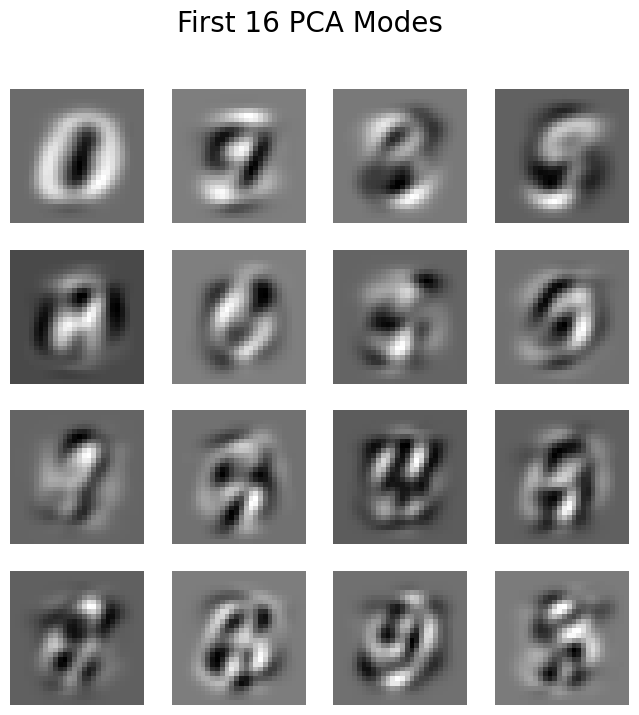
\includegraphics[width=\textwidth]{16_PCA.png}
        \caption{First 16 PCA modes for MNIST dataset}
        \label{fig:pca_modes}
    \end{subfigure}
    \hfill
    % Second subfigure
    \begin{subfigure}[b]{0.45\textwidth}
        \centering
        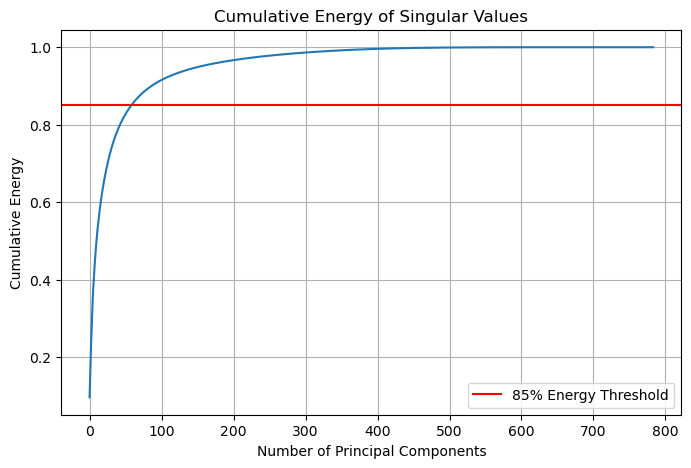
\includegraphics[width=\textwidth]{Cumulative.png}
        \caption{}
        \label{fig:energy}
    \end{subfigure}
    \caption{Cumulative energy captured by PCA modes to achieve $85\%$}
    \label{fig:pca_energy}
\end{figure}

From the image below, it is easy for the human eye to deduce what some numbers shown are, for example the first number being $0$, and the one to the right being $9$. But as we continue some numbers do seem to get more complicated and difficult to identify. This is because of the cumulative energy that had to be captured was $85\%$, and in the figure above we can see that it could be done with only $k = 59$ modes.

Following up, we also wanted to inspect some digit images reconstructed from $59$ truncated PC modes and compare them to the original images to make sure that the image reconstruction was reasonable.

\begin{figure}[H]
    \centering
    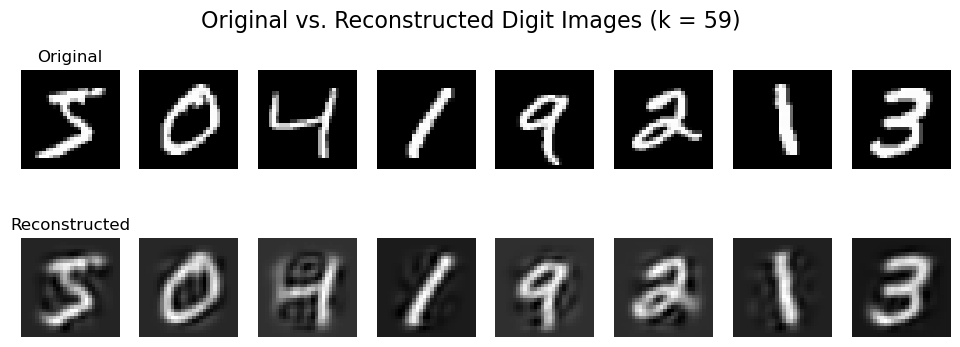
\includegraphics[width=0.6\textwidth]{OGvsReconstructed.png}
    \caption{Few of the original digits and its reconstructed images using $59$ PC modes}
    \label{fig:reconstruction}
\end{figure}

Now we can tell that for sanity check purposes, the reconstructed images are quite similar to the original images, and the PCA modes are capturing the important features of the images.



Moving on, we now test our current methods of digit classification and choose the digits $1, 8$ specifically, and project the data onto the $59$ PC modes. We then train a Ridge classifier on this data and evaluate the test accuracy after performing cross-validation with $5$ folds. The resulting heatmap where the correct digits are displayed on the diagonal and the misclassified digits are displayed off the diagonal is shown below.

\begin{figure}[H]
    \centering
    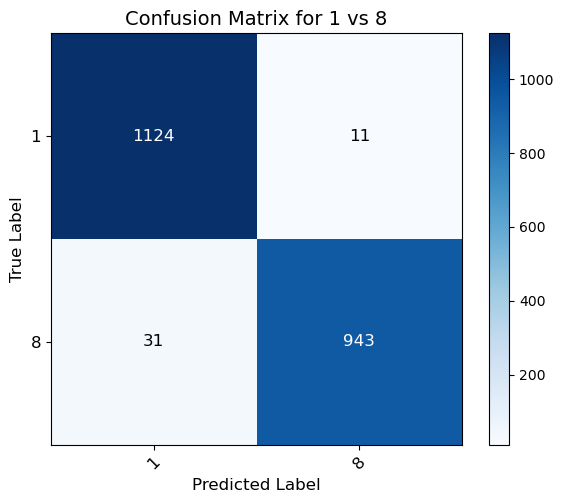
\includegraphics[width=0.45\textwidth]{Confusion1v8.png}
    \caption{Heatmap for binary classification of digits $1, 8$}
    \label{fig:1vs8}
\end{figure}

Similarly, in this assignment we also study the digits $3, 8$ and $2, 7$ and display the heatmaps for these digit pairs side by side below.

\begin{figure}[htbp]
    \centering
    % First subfigure
    \begin{subfigure}[b]{0.45\textwidth}
        \centering
        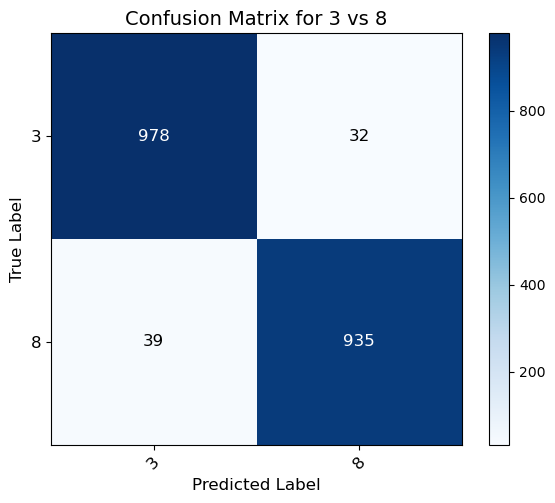
\includegraphics[width=\textwidth]{Confusion3v8.png}
        \caption{Heatmap for classification of digits $3, 8$}
        \label{fig:subfig1}
    \end{subfigure}
    \hfill
    % Second subfigure
    \begin{subfigure}[b]{0.45\textwidth}
        \centering
        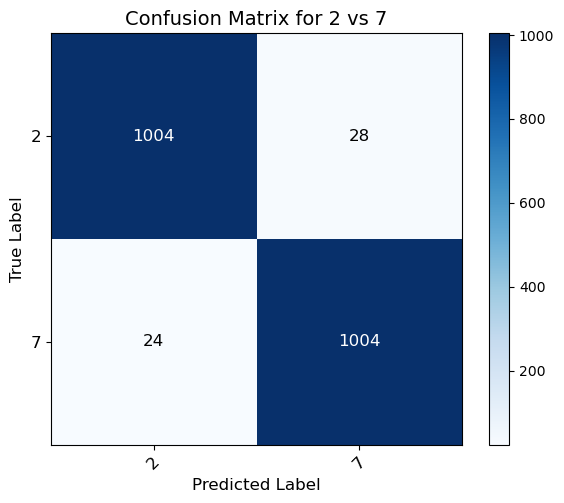
\includegraphics[width=\textwidth]{Confusion2v7.png}
        \caption{Heatmap for classification of digits $2, 7$}
        \label{fig:subfig2}
    \end{subfigure}
    
    \caption{Heatmaps for binary classification of digits $3, 8$ and $2, 7$}
    \label{fig:side-by-side}
\end{figure}

So the good thing is we can clearly see that our Ridge Regression algorithms work with cross-validation. But how good? To analyze deeper we look at the table below that holds the accuracy percentages for the binary classification of the digit pairs $1, 8$, $3, 8$ and $2, 7$. We analyze the Cross-Validation Accuracy, and the Test Accuracy for each of the digit pairs.

\begin{table}[H]
    \centering
    \begin{tabular}{|c|c|c|c|}
    \hline
    \textbf{Digit Pair} & \textbf{Cross-Validation Accuracy} & \textbf{Test Accuracy} \\ \hline
    1, 8               & 0.964                               & 0.980                  \\ \hline
    3, 8               & 0.959                               & 0.964                  \\ \hline
    2, 7               & 0.980                               & 0.975                  \\ \hline
    \end{tabular}
    \caption{Accuracy percentages for binary classification of digit pairs}
    \label{tab:binary_accuracy}
\end{table}

From the table above we see that the competition is very close between the two classifiers, so as a tiebreaker, we implement a multi-class classification for all the digits $0-9$ using both Ridge and KNN classifiers. We then perform cross-validation and evaluate the test accuracy for both classifiers. The results are shown in the table below and heatmap for the confusion matrix is shown below. For optimizing space, I have only shown the heatmap for the KNN classifier.

\begin{figure}[htbp]
    \centering
    \begin{minipage}[b]{0.45\textwidth}
        \centering
        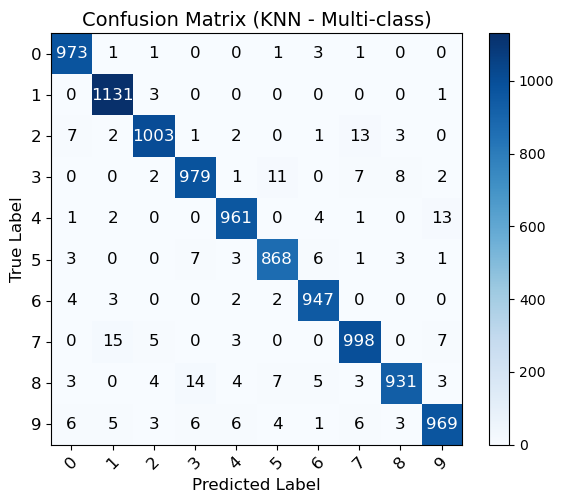
\includegraphics[width=\textwidth]{ConfusionKNN.png}  % Your figure here
        \caption{Confusion Matrix for KNN Classifier}
        \label{fig:KNN_Confusion}
    \end{minipage}
    \hfill
    \begin{minipage}[b]{0.45\textwidth}
        \centering
        \begin{tabular}{c|c|c}
            \hline
            Accurarcy & RR (Multi-class) & KNN (Multi-Class) \\
            \hline
            CV & 0.844 & 0.975 \\
            Test & 0.856 & 0.976 \\
            \hline
        \end{tabular}
        \caption{Ridge Regression and KNN Classifier Accuracy}
        \label{tab:mytable}
    \end{minipage}
\end{figure}



\section*{Summary and Conclusions}

In summary and conclusion, we have successfully implemented a digit classification system using PCA for dimensionality reduction and Ridge regression and KNN classifiers for binary and multi-class tasks. The results show that the Ridge classifier performs well in binary classification tasks, with accuracies above 95\% for all digit pairs. The multi-class classification task also yields high accuracy, with the KNN classifier slightly outperforming the Ridge classifier. The results demonstrate the importance of feature engineering and model selection in image classification tasks, and the trade-offs between computational efficiency and accuracy. Future work could explore more advanced classifiers and feature extraction techniques to further improve classification performance.

\section*{Acknowledgements}

The author is thankful to Professor Frank for providing the materials and resources needed to complete this assignment. The author is also thankful to the peers Eric Ye and Chenab for discussion and implementation of visualization techniques in Python.

\bibliographystyle{abbrv}
\bibliography{references}

\end{document}